\documentclass[a4paper]{article}

\usepackage[english]{babel}
\usepackage[utf8x]{inputenc}
\usepackage{amsmath}
\usepackage{graphicx}
\usepackage[colorinlistoftodos]{todonotes}
\usepackage{booktabs}
\usepackage{tabulary}
\usepackage{multirow, array} % para las tablas
\usepackage{float} % para usar [H]
\usepackage{hyperref}

\title{\Huge{Imagelib} \\ \large{The image processing library for c++} \vspace{0.5cm}\\ \hrule}
\author{
\begin{tabular}{l l}
Erick Eduarte Rojas & B22305\\ 
Fabián Meléndez Bolaños & B24056\\
Luis Felipe Rincón Riveros & B25530
\end{tabular}
}

\begin{document}
\maketitle

\begin{abstract}
\hspace{0.5cm}
	\hrule
    
\hspace{0.7cm}

This document represents a tecnical report for the image processing library "imagelib" developed for c++. You will find basic definitions for image processing elements and filters

\hspace{0.7cm}
	\hrule

\hspace{0.5cm}

	\end{abstract}

\section{Introduction}

This project proposes to create a library in the c++ programming language, which will perform basic functions of image filtering. Especially monochromatic, but it is also planned to be implemented for RGB images.

An image is the set of elements of a two-dimensional function, where (x, y) are spatial coordinates, each pair of coordinates also has an amplitude of f, called intensity or gray level of the image. If the values of (x, y) and amplitude are all finite, we say that the image is a digital image. Digital images are composed of picture elements which commonly are called pixels.

The digital image processing refers to the set of techniques applied to digital images in order to improve quality or facilitate the provision of information. Some of the image processing goals are: smooth the image to remove noise, to enhance the edges and detecting the edges, etc. Usually to achieve them using filters, which can be in the space domain and in the frequency domain.
Among the main applications that have digital image processing is the improvement of pictorial information for human interpretation and facilitate the storage, data transmission and representation for autonomous machine perception.

The focus of this work is to develop a library that is able to apply some of the basic functions of digital processing, in order to apply a filter to an image, to facilitate the understanding and management of information in them.
\section{Objectives}
	\subsection{General}

		\begin{itemize}

		\item To Create a library able to manage certain basic functions in the digital image processing, developed in c++.

		\end{itemize}

	\subsection{Specific}

		\begin{enumerate}
     
        	\item{Learn about image handling in c++.}

			\item{Implement functions of basic operations filters.}

			\item{Implement Smoothing filters in the spatial domain.}
            
            \item{Implement Sharpening filters in the spatial domain.}
            
            \item{Implement dot to dot transformations.}
            
            \item{Implement histogramas analizing functions.}

		\end{enumerate}
\section{Justification}

The digital image proccesing represents an important field for the development of different areas. This is because it becames possible to extract and obtain information that can be manipulated. Of course, it becames necessary to devolps functions that allows to simulate the human vision perception and also perceives hidden data that for the human is impossible to recognize with their visual sense. However, the image computing can operate on images and preform different functions.

It is possible to distinguish three different work areas on digital processing, each of them solving more complex algorithms. First is the basic manipulation of pictures wich involves primitive operations such as image preprocessing to reduce noise, contrast enhancement and image shapering.This process is characterized by the fact that both its inputs and outputs are images. Those basic operations represents important tools for devolp more complex image treatments, therefore there is a middle level wich covers tasks such as partioning an image into regions or objects, description of those objects to reduce them to a form of siutable for computing processing,  and classification of individual objects. The last level of processing compiles the other two to make possible the interpretation of an ensamble of reconized objects, as in image analysis, and preforming the cognitive functions normally associated with vision.

Nowdays there is almost no area of technical endeavor that is not impacted in some way by digital image processing. Those areas of application are pretty diverse. A simple example is the categorize of images according to their souce, like the ones on electromacnetic (EM) energy spectrum, acoustic, ultrasonic and electronic. 
An important case of the images on the EM espectrum are the Gamma-ray images wich are used in nuclear medicine and has the same objective of the X-rays, wich are used to medical diagnostics but also in the industry and other areas like astronomy. Other case are the imaging in the Utraviolet Band where the applications are varied, they include lithography, industrial inspection, microscopy , laser, biological imaging and astronomic observations. The imaging in the visible and infrared bands is the most familiar in all our activities and there are countless applications.

Sumarizing, digital image processing involves task from extract attributes from pictures, to the recognition and interpretation of individual objects. For that reason we considered important to create a library that can represent the basic tools is needed to devolp future applications and the possibility to solve more complex algorithms by treating the data proportionated by the Image library. 



\section{Theoretical Framework}

There are several terms that we believe were important to the development of this library, so, in this section you'll find a brief description for some of them, and in some cases the mathematical background for some of the functions included in this library. Terms like image, digital image, image processing, filter and some filters definitions are found in this section.

An image is a visual representation of an object and it's bidemensional. It is possible to represent with a function dependent of two variables (x and y) wich correspond the spacial coordenates of an amplitud (f) wich is called pixel intensity. A digital image is define when the magnitud of x, y and amplitud are finite and discret amounts.

The digital image contains a fixed number of rows(M) and columns(N) of pixels. Pixels are the smallest individual element of an image, holding quantized values that represent the brightness of a given color at any specific point. This definition allows to write the completere MxN digital image in the following matrix form: \\

\begin{center}
\begin{math}
	\centering
	f(x,y)=
   \begin{pmatrix} 
    f(0,0) & f(0,1) & ... & f(0,N) \\ 
 	f(1,0) & f(1,1) & ... & f(1,N) \\
	\vdots & \vdots & \ddots & \vdots \\
    f(M,0) & (M,1) & ... & f(M,N) \\
   \end{pmatrix}
\end{math}\\
\end{center}

The right side of this equation is by definition a digital image. Each element of this matrix array is a pixel.This image has width M and height N. 

In our library repeatedly we find terms such as width, height, depth, and spectrum. These are the dimentions of the images, each one corresponds to a measure of an amount of pixels in each dimention. The width is the amount of pixels distribuited horizonatally, the height is the amount of pixels vertically, and the depth corresponds to the layers of images, this one is frequently just one layer, except in 3D images; finally the spectrum is the number of color channels in the image, in a monocroatic image, the spectrum is one, and RGB images the spectrum takes a value of three.


The field of digital image processing refers to processing digital images by means of a digital computer. This can be divided in three types of computerized process:low, mid and high.Low-level precesses involve primitive operaion such as image processing to reduce noise, contrast enhancement and image shapering.this level is chatracterized by the both, inputs and outputs, are digital images.Mid-level involves task as segmentation, processing and classification of attributes of the images.The high-level involves"making sense" of an esemble of reconized objects and preforming the cognitive functions normally associated with vision. This library will focus on the low-level of digital image processing.

Also, another therm largely used in this library is filter.Image filtering allows you to apply various effects on pictures, and filter can be seen mathematically as a convolution between two surfaces, one is the image itself and the other a kernel with certain weights.  Arithmetically a filter can be seen as the result of assigning each pixel, the sum of the pixels in the neighborhood for a certain weight. This results in an image which can reduce sudden changes in intensity, or may be increased, the filters can be applied in the frequency domain or the spatial domain. 

If a filter is seen as a convolution, it is usefull to describe some filters with a mask or kernel. This mask is a odd dimention matrix, that determines the weights by which the pixels of the neighborhood are multiplied.

For example, a $3x3$ kernel like this:
\begin{center}
\begin{math}
\begin{pmatrix}
	z_1 & z_2 & z_3 \\
    z_4 & z_5 & z_6 \\
    z_7 & z_8 & z_9 \\
\end{pmatrix}
\end{math}
\end{center}

Will produce a filter that applied to the $(x,y)$ position will produce this:
\begin{center}
\begin{math}
	g(x,y) = f(x-1,y-1)\cdot z_1 + f(x, y-1) \cdot z_2 + f(x+1,y-1)\cdot z_3 + f(x-1, y) \cdot z_4 + f(x,y) \cdot z_5 + f(x+1,y) \cdot z_6 + f(x-1, y+1) \cdot z_7 + f(x, y+1) \cdot z_8 + f(x+1, y+1) \cdot z_9
\end{math}
\end{center}

Usually, the result of the convolution is multiplied or divided by a constant to avoid loss of information or exceeding storage capability.

There two different types of filters, the ones managed on the frequency domain because they use the Fourier transform, and the spacial filters. The last ones consists simply of moving the filter mask from point to point in an image.The response of the filter at each pixel is calculated by a predefined relationship. For linear spatial filtering  the response is given by a sum of products of the maks coefficients and the corresponding pixel values of the image. The size of the mask or kernel mxn are assumed to be both impair numbers.

There are also nonlinear spatial filter that also operates on neighborhoods and the mechanincs of sliding a mask but with non linear functions, for example the median, the modal, the variance and among others.

In this library, some filters were implemented, below you'll find the theoretical support of most of them.

\subsection{Arithmetic functions}

\subsubsection{Image subtraction}
The subtraction of two images subtract the pixel values of two images with the same dimensions, is useful to detect the differences between two images. 

\subsubsection{Multiply image}
Multiply an image by a factor is used to increase od decrease the value of the intensity of all the pixels in the image.

\subsubsection{Binarize image}
To binarize an image is necesary a cutoff intensity value, all the values below this intensity is set to 0 and all the pixel values higher than this cutoff intensity is set to the maximun value in RGB case the maximum is 255.


\subsection{Sharpening spatial filters}
The principal objective of sharpening is to highlight fine detail in an image or to enhance detail that has been blurred, either in error or as a natural effect of a particular method of image acquisition. Uses of image sharpening vary and include applications ranging from electronic printing and medical imaging to industrial inspection and autonomous guidance in military systems.
Since averaging is analogous to integration, it is logical to conclude that sharpening could be accomplished by spatial differentiation. Fundamentally, the strength of the response of a derivative operator is proportional to the degree of discontinuity of the image at the point at which the operator is applied. Thus, image differentiation enhances edges and other discontinuities (such as noise) and de-emphasizes areas with slowly varying gray-level values.

\subsubsection{Lapacian filter}
The derivative of an image is defined in terms of diferences, therefore, a second derivative also is defined in terms of diferences between pixel values. Most sharpening filters work with derivatives. The Laplacian filter is defined by the second derivative. THe mathematical aproach is given by:
\begin{math}
\nabla^2 f = \frac{\partial^2 f}{\partial x^2} + \frac{\partial^2 f}{\partial y^2} 
\end{math}

Then, we can define the derivative $\frac{\partial f}{\partial c} = f(x+1) -f(x) $, and taking this aproach, and defining the laplacian filter as:
\begin{math}
g(x,y) = f(x,y) + \nabla^2f(x,y)
\end{math}
\\
We can define a Laplacian mask as: 
\begin{center}
\begin{math}
   \begin{pmatrix} 
   0 & 1 & 0 \\ 
   1 & -4 & 1 \\
   0 & 1 & 0 \\ 
   \end{pmatrix}
\end{math}
\end{center}

This mask represents a second derivative in x and a second derivative in y summed, just like the laplacian definition. But we can expand the laplacian definition to include the diagonal directions, and have a full laplacian mask, like this one: \\
\begin{center}
\begin{math}
   \begin{pmatrix} 
   1 & 1 & 1 \\ 
   1 & -8 & 1 \\
   1 & 1 & 1 \\ 
   \end{pmatrix}
\end{math}\\
\end{center}
The laplacian filter enhances the edges in all directions (the results obtained can be considered as a "sum" of those obtained after applying a series of edge enhacenment models). As a negative attribute, the Laplacian filter reacts greatly to noise, so its recomended to apply a smoothing filter first, in case ist been used to enhance edges.  \\

\subsubsection{Gradient}
First derivatives in image processing are implemented using the magnitude of
the gradient. For a function $f(x, y)$, the gradient of $f$ at coordinates $(x, y)$ is defined as the two-dimensional column vector: \\
\begin{center}
\begin{math}
 \nabla f(x,y) =
 \begin{pmatrix} 
  \frac{\partial f}{\partial x} \\
  \frac{\partial f}{\partial y} \\
  \end{pmatrix}
\end{math}
\end{center}
The Gradient is approximate by the diference in magnitude of the two gradients (x and y). A simplified aproximation is the sobel masks, that are represented by:
\begin{center}

\begin{math}
   \begin{pmatrix} 
   1 & 0 & -1 \\ 
   2 & 0 & -2 \\
   1 & 0 & -1 \\ 
   \end{pmatrix}
\end{math}  \& 
\begin{math}
   \begin{pmatrix} 
   1 & 2 & 1 \\ 
   0 & 0 & 0 \\
   -1 & -2 & -1 \\ 
   \end{pmatrix}
\end{math}\\
\end{center}
The idea behind using a weight value of 2 is to achieve some smoothing by giving more importance to the center point.

\subsubsection{Prewitt}
Technically, it is a discrete differentiation operator, computing an approximation of the gradient of the image intensity function. At each point in the image, the result of the Prewitt operator is either the corresponding gradient vector or the norm of this vector. The Prewitt operator is based on convolving the image with a small, separable, and integer valued filter in horizontal and vertical direction and is therefore relatively inexpensive in terms of computations. On the other hand, the gradient approximation which it produces is relatively crude, in particular for high frequency variations in the image. The Prewitt operator was developed by Judith M. S. Prewitt.\\

In this library were implemented four masks of Prewitt for different direcntion  gradients: North-South (N-S), Northwest-Southeast (NW-SE), East-West (E-W), Southwest-Northeast (SW-NE). This are the masks implemented: \\
\begin{center}
\ \ N-S: \begin{math}
   \begin{pmatrix} 
   1 & 1 & 1 \\ 
   0 & 0 & 0 \\
   -1 & -1 & -1 \\ 
   \end{pmatrix}
\end{math} ,\ \ \ \  E-W:
\begin{math}
   \begin{pmatrix} 
   1 & 0 & -1 \\ 
   1 & 0 & -1 \\
   1 & 0 & -1 \\ 
   \end{pmatrix}
\end{math},  \\ SW-NE: \begin{math}
   \begin{pmatrix} 
   0 & -1 & -1 \\ 
   1 & 0 & -1 \\
   1 & 1 & 0 \\ 
   \end{pmatrix}
\end{math},  NW-SE: \begin{math}
   \begin{pmatrix} 
   1 &1 & 0 \\ 
   1 & 0 & -1 \\
   0 & -1 & -1 \\ 
   \end{pmatrix}
\end{math}\\
\end{center}

\subsubsection{Filter edge enhancement by displacement}

Its a sharpening spatial transformation. Uses displacement and subtraction tecniques to enhance the edges in images. When the original image is displaced, the intensity of the displaced pixel minus the intensity of the non displaced pixel, deemphasizes low contrast areas, and enhance high contrast areas, as a result the transformed image presents  in its majority the edges of the original image.

\subsubsection{Horizontal and Vertical Borders Enhancement}

As said before, most sharpening spatial filters uses derivatives as theri mathematical support. These kind of filters use derivatives as well, and can be seen as derivatives in the x direction (for the horizontal edges enhancement) and in the y direction (for the vertical edges enhancement).

These filters masks look like this:\\
\begin{center}
	Horizontal Edges Enhancement: 
 \begin{math}
   \begin{pmatrix} 
   0 & 0 & 0 \\ 
   1 & 0 & -1 \\
   0 & 0 & 0 \\ 
   \end{pmatrix}
\end{math},  \\ Vertical  Edges Enhancement:\ \ \ \  \begin{math}
   \begin{pmatrix} 
   0 & 1 & 0 \\ 
   0 & 0 & 0 \\
   0 & -1 & 0 \\ 
   \end{pmatrix}
\end{math}\\
\end{center}

\subsection{Smoothing spacial filters}

\subsubsection{Median filter}

The median filter uses a kernel to calculate the median of the pixel values, in this way the intensity is homogenized .First is necessary to order the pixel values in order ascendant or descendant and then choose the middle one to stablish it on the central pixel.
This filter allows to reduce the noise on an image , for example the salt\&pepper effect, without blurring the image but losing resolution.



\subsubsection{Average filter}

The average filter uses a kernel, a small part of the image and subtracs the pixel values. With those values it calculates the average and sets it into the center pixel of the kernel. This filter is used to smooth the picture by reducing the abrupt change of pixel values on the surroundings. The average is difined by:\\

\begin{center}
\begin{math}
Average= \frac{\sum \limits_{i=0}^{N}\!\!(x_i)}{N}
\end{math}
\end{center}


\subsubsection{Modal filter}

The modal filter calculates the modal value of a certain pixel values subtracted by the kernel, it means that the central pixel is set with the most frequent value. If all the values are different this filter sets the average value.

\subsubsection{Gaussian filter}

A Gaussian filter is a 2-D convolution operator that is used to smoothes an image and remove detail and noise by calculating weighted avereges in a kenerl using the next expression:\\

\begin{center}
\begin{math}
G_{\sigma}(x,y)=\frac{1}{\sqrt{2\pi\sigma^2}}e^\frac{x^2+y^2}{2\sigma^2}
\end{math}
\end{center}
Where coordenates x,y are coordenates of the kernel located on arbitrary pixel positions in a bitmap image. Is used to take the mask center as the point (0,0).For example, a filter 3x3 with singular standard desviation ($\sigma=1$) would have the next kernel:

\begin{center}
\begin{math}
\begin{pmatrix} 
   0.1467 &0.2420 & 0.1467 \\ 
   0.2420 & 0.3999 & 0.2420 \\
   0.1467 & 0.2420 & 0.1467 \\ 
\end{pmatrix}
\end{math}\\
\end{center}

\subsection{Dot to dot transformations}


\subsubsection{Dynamic dilatation}

The dilatation of the dynamic range is used in images poorly contrasted, to stand out the range of intensity that predominates in the image. This method uses three ranges of pixel values, and applies the transformation:\\ 
\\
\begin{math}
v= \left\{
	\begin{array}{cl}
		u\alpha & \mbox{si } 0<u<a\\
		\beta(u-a)+v_a &\mbox{si } a\leq u<b\\
	\gamma(u-b)+v_b &\mbox{si } b\leq u\leq L\\
	\end{array}\right.
\end{math}
\\
\\
With $\alpha$, $\beta$ and $\gamma$, real numbers, L is the 
value of intensity, a and b are the cutoff pixel values, u is the actual intensity value that will be transformed in v, and $v_a$ and $v_b$ are the pixel values in a and b already dilatated.
The values of a and b can be obtained by observing the histogram, between $\left[a,b\right]$ the transformation increase more this pixel values than the other ranges.
\subsubsection{Inverse}

The inverse of an image calculates the substraction of all the pixel values and the maximum value (255 to RGB), and set the new image with these pixel values.

\subsubsection{Logarithmic transfomation}
This transformation maps a narrow range of low gray-level values in the input image into a wider range of output levels.The opposite is true of higher values of input levels. We would use a transformation of this type to expand the values of dark pixels in an image while compressing the higher-level values.
It performs a logarithmic transformation given by the ecuation:
\begin{center}
	$v = c \cdot log (u + 1)$
\end{center}
Where $v$ is the transformed pixel's intensity, $u$ the original image's pixel's intensity, and $c$ is a constant to normalize the transformed value.
\subsubsection{Color slicing}

Color slicing a color image processing, thus can be used in monocromatic images. It consists in taking two color values and assing a neutral value to any pixel that isn't between those color values. The result is an image that enhances the some colors, and de-emphasizes the rest of color values. 


\section{Power-Law Transformation}

Its similar to the logarithmic transformation, it narrows a range of high gray-level values in the input image into a wider range of output levels. Mathematically it calculates the following function:
\begin{math}
g(x,y) = k \cdot \left( f(x,y) )^{\gamma} \right)
\end{math}



\subsection{Histogram \& Equalization }
\subsubsection{Histogram}

In statistics, an histogram is a graphical representation of the distribution of data. It is an estimate of the probability distribution of a continuous variable. A histogram is a representation of tabulated frequencies, shown as adjacent rectangles, erected over discrete intervals. In an image a histogram is a type of histogram that acts as a graphical representation of the tonal distribution in a digital image. It plots the number of pixels for each tonal value. By looking at the histogram for a specific image a viewer will be able to judge the entire tonal distribution at a glance.

\subsubsection{Equalization}

Histogram equalization is a method in image processing for contrast adjustment using the image's histogram, This method usually increases the global contrast of many images, especially when the usable data of the image is represented by close contrast values. Through this adjustment, the intensities can be better distributed on the histogram. This allows for areas of lower local contrast to gain a higher contrast. Histogram equalization accomplishes this by effectively spreading out the most frequent intensity values. The method is useful in images with backgrounds and foregrounds that are both bright or both dark

\subsection{Other transformations}
\subsubsection{Filter order stadisics}

Order-statistics filters are nonlinear spatial filters whose response is based on ordering (ranking) the pixels contained in the image area encompassed by
the filter, and then replacing the value of the center pixel with the value determined by the ranking result.
Its a general purpose transformations, it roams the neighborhood, and orders the pixel intensities in a increasing order, and takes the value for the transformed image's pixel as the $k_{th}$ order of intensity.
There are well known particular cases of this transformation, as the median filter, maximun or minumun filters.

\subsubsection{Kirsch masks}

The edge detection is very used in digital image processing, the edges in an image are those areas where the intensity value has a  transition of high to low intensity or low to high. One of the methods to detect the edges is to apply the Kirsch masks, there are 8 Kirsch masks, to detect the edges in 8 different directions, the masks that apply the same filter in different directions are named steering filters or oriented filters. These Kirsch masks are gived by:\\
\begin{centering}
\ \ \ \ \ \ \ \ 0 degrees: \begin{math}
   \begin{pmatrix} 
   -3 & -3 & 5 \\ 
   -3 & 0 & 5 \\
   -3 & -3 & 5 \\ 
   \end{pmatrix}
\end{math} ,\ \ \  45 degrees: \begin{math}
   \begin{pmatrix} 
   -3 & 5 & 5 \\ 
   -3 & 0 & 5 \\
   -3 & -3 & -3 \\ 
   \end{pmatrix}
\end{math}\\
90 degrees: \begin{math}
   \begin{pmatrix} 
   5 & 5 & 5 \\ 
   -3 & 0 & -3 \\
   -3 & -3 & -3 \\ 
   \end{pmatrix}
\end{math}, 135 degrees: \begin{math}
   \begin{pmatrix} 
   5 & 5 & -3 \\ 
   5 & 0 & -3 \\
   -3 & -3 & -3 \\ 
   \end{pmatrix}
\end{math}\\

\ 180 degrees: \begin{math}
   \begin{pmatrix} 
   5 & -3 & -3 \\ 
   5 & 0 & -3 \\
   5 & -3 & -3 \\ 
   \end{pmatrix}
\end{math},\ \  225 degrees: \begin{math}
   \begin{pmatrix} 
   -3 & -3 & -3 \\ 
   5 & 0 & -3 \\
   5 & 5 & -3 \\ 
   \end{pmatrix}
\end{math}\\

270 degrees: \begin{math}
   \begin{pmatrix} 
   -3 & -3 & -3 \\ 
   -3 & 0 & -3 \\
   5 & 5 & 5 \\ 
   \end{pmatrix}
\end{math}, 315 degrees: \begin{math}
   \begin{pmatrix} 
   -3 & -3 & -3 \\ 
   -3 & 0 & 5 \\
   -3 & 5 & 5 \\ 
   \end{pmatrix}
\end{math}\\
\end{centering}

\subsubsection{Freeman masks}

The Freeman masks are a group of masks that apply the same filter rotated, a steering filter, steerable filters may be designed in quadrature pairs to allow adaptive control over phase as orientation, each of the Freeman masks allows to detect borders in different directions, there are 8 masks that are given by:\\
\\
\begin{centering}
mask 0: \begin{math}
   \begin{pmatrix} 
   1 & 1 & 1 \\ 
   1 & -2 & 1 \\
   -1 & -1 & -1 \\ 
   \end{pmatrix}
\end{math}, mask 1: \begin{math}
   \begin{pmatrix} 
   1 & 1 & 1 \\ 
   -1 & -2 & 1 \\
   -1 & -1 & 1 \\ 
   \end{pmatrix}
\end{math}\\

\ mask 2: \begin{math}
   \begin{pmatrix} 
   -1 & 1 & 1 \\ 
   -1 & -2 & 1 \\
   -1 & 1 & 1 \\ 
   \end{pmatrix}
\end{math}, mask 3: \ \begin{math}
   \begin{pmatrix} 
   -1 & -1 & 1 \\ 
   -1 & -2 & 1 \\
   1 & 1 & 1 \\ 
   \end{pmatrix}
\end{math}\\

mask 4: \begin{math}
   \begin{pmatrix} 
   -1 & -1 & -1 \\ 
   1 & -2 & 1 \\
   1 & 1 & 1 \\ 
   \end{pmatrix}
\end{math}, mask 5: \begin{math}
   \begin{pmatrix} 
   1 & -1 & -1 \\ 
   1 & -2 & -1 \\
   1 & 1 & 1 \\ 
   \end{pmatrix}
\end{math}\\

\ mask 6: \begin{math}
   \begin{pmatrix} 
   1 & 1 & -1 \\ 
   1 & -2 & -1 \\
   1 & 1 & -1 \\ 
   \end{pmatrix}
\end{math},\  mask 7: \begin{math}
   \begin{pmatrix} 
   1 & 1 & 1 \\ 
   1 & -2 & -1 \\
   1 & -1 & -1 \\ 
   \end{pmatrix}
\end{math}\\
\end{centering}
\subsubsection{Maximum \& Minimum filters}

These are pretty simple filters, they roam the pixel's neighborhood, and choose the maximun or minimun value. Can be used as smoothing filters, but their results arent exactly the ones of an smoothing filter, yet they can help to reduce noise. These filters are particular cases of the order-statistics filter.

\subsubsection{Variance}

In probability and statistics, the variance is a measure of how far a set of numbers is spread out. In other words, if the variance is zero all the values are equals; if the variance is small, it means the vales are very likely and close  to the mean; and if the variance is high, that indicates that the data points are very spread out from the mean form each other.

In this case the variance is about pixel values arround a kernel that goes trought the image, it mean those values can be equally likely, the variance of those n values can be calculated by the formula: \\

\begin{center}
\begin{math}
Var(x)= \frac{\sum \limits_{i=0}^{N} (\bar x - x_i)^2}{N}
\end{math}
\end{center}

\subsubsection{Covariance}

The covariance, calculates the covariance matrix of an image. This function calculates something similar to the function below: \\
\begin{math} 
	g(x,y) = \sum \limits_{n=0}^{N} \sum \limits_{m=1}^M \left( f(x,y) - \overline{f(x,y)}\right)\left(f(x + \Delta x, y + \Delta y) - \overline{f(x + \Delta x, y + \Delta y)} \right)
\end{math}
Where it calculates the variation between two series, one is the normal one, and the other is displaced by two parameters $\Delta x$ \& $\Delta y$. For an image it its calculated for a neighborhood.

\subsection{Correlogram}
Its the Image co\-ocurrence matrix.It is a matrix or distribution that is defined over an image to be the distribution of co-occurring values at a given offset. Mathematically, a co-occurrence matrix $C$ is defined over an $n x m$ image I, parameterized by an offset $(\Delta x,\Delta y)$, as:


\begin{math}
 C_{\Delta x,\Delta y}(i,j) = \sum \limits_{p=1}^{n} \sum \limits_{q=1}^{m} 
 \left\{
	\begin{array}{l l}
		1  & \mbox{if } I(p,q)=i \mbox{  and } I(p+\Delta x,q + \Delta y)= j \\
		0 & \mbox{Otherwise}
	\end{array}\right.
\end{math}
\subsubsection{RGB to gray scale}

To convert a RGB image to monochromatic is necessary to mix in a linear proportion the channels red ,green and blue of the picture matching the luminance of the grayscale image to the luminance of the color image. This is due the luminance component captures what is most perceived by humans as color in one channel.  

This library uses this covertion:

\begin{center}
\begin{math}
f(x,y)= 0.11R+0.56G + 0.14B
\end{math}
\end{center}

Where f is the intensity of the pixel on the gray scale and R,G and B the pixel values on the different channels.

\subsection{Noise}

Noise represents unwanted information wich deteriorates image quality.Noise is defined as a process (n) wich affects the acquired image (f) and is not part of the scene (initial signal -s). Using additive noise model, this can be written as:
\begin{center}
\begin{math}
f(i,j)=s(i,j) +n(i,j)
\end{math}
\end{center}

\subsubsection{Gaussian noise}

This additive noise is characterized because the final pixel values represents the ideal values plus certain error. It produces little variations on the image, in fact, the energy spectrum is constant for all the frequencies, it means the intensity of all the pixels is altered.This kind of noise is usually produced by the electronic components.

It can  be described as a gaussian variable tahat follows a normal distribution:\\

\begin{center}
\begin{math}
P(g(x,y)-\sigma < f(x,y) <g(x,y)+\sigma)=70\%
\end{math}
\end{center}

\begin{center}
\begin{math}
P(g(x,y)-2\sigma < f(x,y) <g(x,y)+2\sigma)=90\%
\end{math}
\end{center}



\begin{figure}
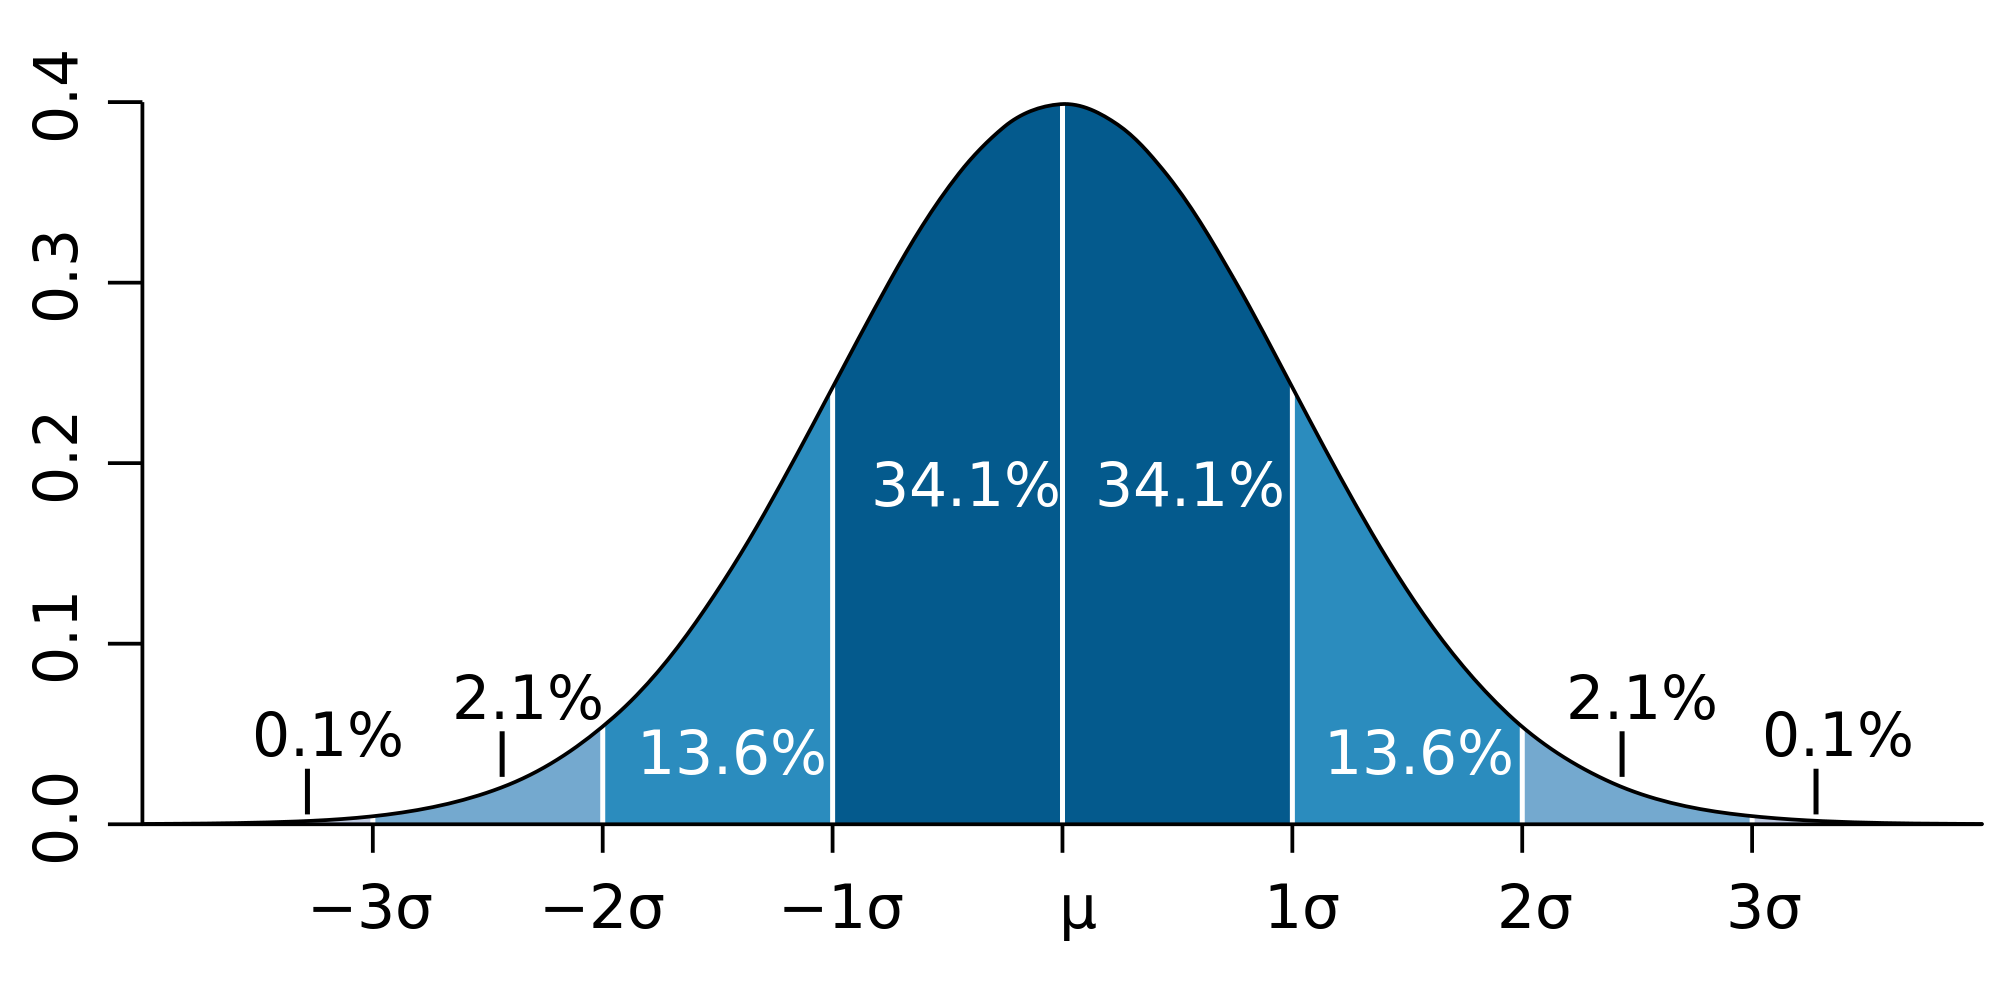
\includegraphics[scale=0.15]{./.Multimedia/Standard_deviation_diagram.png}

\caption{Standard desviation $\sigma$}
\end{figure}


\subsubsection{Salt \& Pepper}

In salt\&pepper noise model there are only two possible values of noise , the one of salt which are the highest intensity (white-salt) and the lowest intensity (black-pepper). The probability of obtaining each of them is less than 0.1 (otherwise, the noise would vastly dominate the image). 


\subsection{Interpolation}
\subsubsection{Closer neighborhood}

Interpolation is the process of calculate numeric values based on others already known by concrete algorithms. The objective is to return a bigger image filling the unknow pixels with the values estimated.
The interpolation of the closer neighborhood consist in basically make bigger the pixel by considering its value.


\section{Design}
	This library is contained in a single file, distribuited in the header file and the cpp file. This is because it contains a single class, the Image class, around which the library is built, and the only class-like abstraction is the Imagelib class. Also it's easier to comprehend its functioning, and allows every function to be a feature of an Image. 
    
    The image class contains a list of functions that can be applied to the image object. The files are structured with a set of Constructors, and a list of set's and get's to the image properties as dimentions and pixel intensity values. Then the rest library consists of a series of filters and transformations to the images, that almost everytime return a Image object with the transformed Image.
    
    Also, in this library, we use the CImg library, in order to handle images, and some basic, complicated and low level functions, like display and  obtain or modify images. This is made, containing a CImg object in the Image class as a global variable. We decided to use the CImg library because is a single file library, so it was easier to wrap some functions and variables. 
    
    The Image Class contains, some variables like the mentioned CImg object, that contains a Image with pixel intensities defined as unsigned chars, this is because an image occupies a large space in memory, since each pixel must be stored in memory; and this way only uses one byte per pixel, and will have 256 levels of intensity, which is greater than can be detected by a human.
    
    For the image dimentions, it's used variables of type unsigned int, since're the type of variable used in the library CImg. 
    You can find the whole Image Class diagram in the following tables.
    
\begin{table}[H]
	\label{UML}
    \caption{UML Diagram}
	\centering
    
	\begin{tabular}[15cm]{ 
    >{\arraybackslash}m{15cm}}
        \toprule 

		\large{Image Class} \\   

		\midrule
		
       	- width : unsigned int\\
        - height : unsigned int \\
        - depth : unsigned int\\
        - spectrum : unsigned int \\
        - Img : CImg<unsigned char> \\

        \midrule
        + Image() : void \\
        + Image(const char*) : void \\
        + Image(unsigned int, unsigned int, unsigned int, unsigned int, unsigned char) : void \\
        + ~Image() : void \\
        + get\_width() : unsigned int \\
        + get\_height() : unsigned int \\
        + get\_spectrum() : unsigned int \\
        + get\_depth() : unsigned int \\
        + save(const char *const) : void \\
		+ display(const char*) : void \\
        + get\_pixel\_value(int, int, int, int) : unsigned int \\
		+ set\_pixel\_value(int, int, int, int, unsigned char): void \\
        + substract\_img(Image) : Image \\
		+ sum\_img(Image) : Image \\
		+ multiply\_img(double) : Image \\
		+ binarize\_img(unsigned int) : Image \\
        + filter\_Laplacian() : Image \\
		+ filter\_Laplacian\_no\_diagonal(): Image	\\
        + filter\_Gradient\_vertical(): Image \\
		+ filter\_Gradient\_horizontal(): Image \\
		+ filter\_Prewitt\_N\_S(): Image 	\\
        + filter\_Prewitt\_NE\_SW(): Image\\
		+ filter\_Prewitt\_E\_W() : Image\\
        + filter\_Prewitt\_NW\_SE(): Image \\
        + filter\_edge\_enhacement\_displacement(unsigned int, unsigned int) : Image\\
        + filter\_horizontal\_borders(): Image \\
        + filter\_vertical\_borders(): Image \\
        + filter\_median(int): Image \\
        + filter\_average(int): Image \\
        + filter\_gaussian(int, int): Image \\
        + filter\_modal(int): Image \\
        + filter\_dynamic\_range\_dilatation(unsigned char, unsigned char, double, double, double): Image \\
        + inverse(): Image \\
        + log\_transformation(): Image \\
        + power\_law\_transformatiom(double exponent): Image \\
        + color\_slicing (unsigned char*, unsigned char*, unsigned char*): Image \\
        + get\_(unsigned int c, unsigned int z) : int*\\
        + plot\_histogram(int, const char* title) : void \\
        + histogram\_equalization(int*, const char* title): int* \\
        
        \bottomrule
        
 
	\end{tabular}
    
\end{table}

\begin{table}[H]
	\label{UML2}
    \caption{UML Diagram, continued}
	\centering
    
	\begin{tabular}[15cm]{ 
    >{\arraybackslash}m{15cm}}
        \toprule 

		\large{Image Class} \\   

		\midrule
 		+ autocovariance(int, int) : CImg<float> \\
		+ plot\_histogram\_equalization(int, const char*) \\
        + filter\_order\_stadistics(int dim, int order) : Image \\
		+ variance(int) : Image \\
        + filter\_kirsch\_0() : Image \\
		+ filter\_kirsch\_45() : Image \\
        + filter\_kirsch\_90() : Image \\
        + filter\_kirsch\_135() : Image \\
        + filter\_kirsch\_180() : Image \\
        + filter\_kirsch\_225() : Image \\
        + filter\_kirsch\_270() : Image \\
        + filter\_kirsch\_315() : Image \\
        + filter\_freeman\_0() : Image \\
        + filter\_freeman\_1() : Image \\
        + filter\_freeman\_2() : Image \\
        + filter\_freeman\_3() : Image \\
        + filter\_freeman\_4() : Image \\
        + filter\_freeman\_5() : Image \\
        + filter\_freeman\_6() : Image \\
        + filter\_freeman\_7() : Image \\
        + filter\_maximum() : Image \\
        + filter\_minimum() : Image \\
        + gray\_scale() : Image \\
        + gaussian\_noise(double) : void \\
        + salt\_pepper(double) : void \\
        + interpolation() : void \\
		+ coorrelogram(unsigned int,unsigned int) : Image \\
		+ coorrelogram\_ZC(unsigned int,unsigned int,unsigned int, unsigned int): Image \\
        \bottomrule
        
 
	\end{tabular}
    
\end{table}

\section{Bibliography}
\begin{enumerate}
\item Gonzalez, Rafael C. \& Woods, Richard E. (2002) . Digital Image Processing . (2nd Ed.). Prentice Hall, New Jersey.

\item González, R.C. \& Wintz, P. (1996), Procesamiento digital de imágenes. Addison Wesley, Tema 3,4, pg 89-269.

\item C. Pinilla, A. Alcalá \& F. J. Ariza. (1997). Filtrado de Imágenes en el Dominio de la Frecuencia. Departamento de Ingeniería Cartográfica, Geodésica y Fotogrametría. Universidad de Jaén. From: \url{ http://www.aet.org.es/revistas/revista8/AET8_5.pdf.}
\end{enumerate}



\end{document}
